\chapter{Resultados e Discussões} \label{ch:RD}

\section{Projeto de Software} \label{sec:PS}

A etapa inicial no desenvolvimento de \textit{software} é compreender os relacionamentos entre o \textit{software} em projeto e o seu ambiente exterior. Esta etapa é essencial porque mostra como se dará a estrutura do sistema para se comunicar com o seu ambiente e quais serão os limites estabelecidos para o mesmo. A definição do sistema informa quais serão as funcionalidades implementadas e os recursos disponíveis \cite{sommerville2011engenharia}.

Os diagramas abordados serão o de caso de uso, de sequência e de atividade. Esses três diagramas proporcionam uma visão geral de cada etapa do funcionamento do sistema. Além disso, será discutido também um modelo de documento referente ao banco de dados adotado.

\subsection{Casos de uso} \label{subsec:casosDeUso}

As interações entre alguns elementos do sistema serão relatadas pelos diagramas de caso de uso seguintes, utilizando de uma abordagem abstrata e sem muitos detalhas de implementação, pois destinam-se apenas à oferecer uma compreensão do que o sistema faz, ou seja, define os requisitos funcionais do sistema \cite{sommerville2011engenharia}.

A figura \ref{img:caso_de_uso_1} mostra o caso de uso referente à utilização da aplicação cliente pelo usuário final, enquanto a figura \ref{img:caso_de_uso_2} demonstra as interações do sistema do ponto de vista da API.

\imagem{0.8}{caso_de_uso_1}{Diagrama de caso de uso referente ao usuário final}{O autor}
\newpage

\textbf{Visualizar dados atuais}

\begin{itemize}
    \item Atores
    \begin{itemize}
        \item Usuário
    \end{itemize}
    
    \item Pré-condições
    \begin{itemize}
        \item o usuário deve estar autenticado
    \end{itemize}

    \item Fluxo de eventos primário
    \begin{enumerate}
        \item o usuário deve efetuar o \textit{login} informando o \textit{username} e a senha;
        \item caso o usuário não seja autenticado, o sistema informa a respeito de credenciais inválidas e encerra o caso de uso;
        \item o usuário é liberado para visualizar os dados atuais dos sensores da estação;
        \item após a visualização o usuário pode finalizar o caso de uso ou efetuar uma nova consulta se desejar.
    \end{enumerate}

    \item Fluxo alternativo
    \begin{itemize}
       \item o usuário desiste de visualizar os dados atuais e cancela o caso de uso clicando no botão voltar.
    \end{itemize}

\end{itemize}

\textbf{Visualizar histórico}

\begin{itemize}
    \item Atores
    \begin{itemize}
        \item Usuário
    \end{itemize}

    \item Pré-condições
    \begin{itemize}
        \item o usuário deve estar autenticado
    \end{itemize}

    \item Fluxo de eventos primário
    \begin{enumerate}
        \item o usuário deve efetuar o \textit{login} informando o \textit{username} e a senha;
        \item caso o usuário não seja autenticado, o sistema informa a respeito de credenciais inválidas e encerra o caso de uso;
        \item a API autentica o usuário;
        \item o usuário é liberado para escolher qual(is) variável(is) e qual período cujo histórico será exibido;
        \item após a visualização do histórico o usuário pode finalizar o caso de uso se desejar.
    \end{enumerate}

    \item Fluxo alternativo
    \begin{enumerate}
        \item após a escolha da(s) variável(is) ou do período de exibição do histórico o usuário pode voltar para a tela anterior e escolher novas variáveis ou um novo período;
        \item o histórico é exibido para o usuário;
        \item após a visualização do histórico o usuário pode finalizar o caso de uso ou efetuar uma nova consulta se desejar.
    \end{enumerate}

    \item Fluxo alternativo
    \begin{enumerate}
        \item o usuário desiste de visualizar o histórico e cancela o caso de uso clicando no botão voltar.
    \end{enumerate}
\end{itemize}

\imagem{0.8}{caso_de_uso_2}{Diagrama de caso de uso do ponto de vista da API}{O Autor}

\textbf{Coletar dados}

\begin{itemize}
    \item Atores
    \begin{itemize}
        \item API
    \end{itemize}

    \item Pré-condições
    \begin{itemize}
        \item conectar-se ao \textit{datalogger}
    \end{itemize}

    \item Fluxo principal
    \begin{enumerate}
        \item a API conecta-se ao \textit{datalogger} e envia comandos seriais (ver Anexo \ref{anex:anexo1}) via \textit{socket} TCP requisitando os dados;
        \item após a resposta do \textit{datalogger}, os dados são tratados;
        \item a API armazena as informações no banco de dados e encerra o caso de uso.
    \end{enumerate}
    
    \item Fluxo alternativo
    \begin{enumerate}
        \item a API não consegue se conectar ao \textit{datalogger}, o caso de uso é cancelado.
    \end{enumerate}
	
	\item Fluxo alternativo
    \begin{enumerate}
        \item a API conecta-se ao \textit{datalogger} e requisita os dados;
        \item a API verifica que os dados do banco já são os mais recentes;
        \item o caso de uso é cancelado.
    \end{enumerate}

    \item Pós-condições
    \begin{itemize}
       \item novas informações estão disponíveis no banco de dados para serem consultadas.
    \end{itemize}
\end{itemize}

\textbf{Servir dados}

\begin{itemize}
    \item Atores
    \begin{itemize}
        \item API
    \end{itemize}

    \item Pré-condições
    \begin{itemize}
        \item verificar quais as variáveis requeridas pela aplicação cliente através dos parâmetros da requisição HTTP.
    \end{itemize}

    \item Fluxo principal
    \begin{enumerate}
        \item a API verifica quais dados foram solicitados pelo cliente;
        \item recupera as informações necessárias no banco de dados;
        \item a API envia os dados para a aplicação e encerra o caso de uso.
    \end{enumerate}

	\item Fluxo alternativo
    \begin{enumerate}
        \item a API verifica quais dados foram solicitados pelo cliente;
        \item a API não consegue se conectar ao banco de dados, então o caso de uso é encerrado.
    \end{enumerate}
    
    \item Pós-condições
    \begin{itemize}
        \item o usuário pode visualizar as informações consultadas.
    \end{itemize}
\end{itemize}

\textbf{Autenticar usuário}

\begin{itemize}
    \item Atores
    \begin{itemize}
        \item API
    \end{itemize}

    \item Pré-condições
    \begin{itemize}
        \item recuperar as credenciais de \textit{login} do usuário na requisição da aplicação cliente.
    \end{itemize}

    \item Fluxo principal
    \begin{enumerate}
        \item a API conecta-se ao banco de dados;
        \item a API verifica que as credenciais do usuário são válidas;
        \item a API responde à requisição de \textit{login} enviando o \textit{token} de acesso do cliente.
    \end{enumerate}

	\item Fluxo alternativo
    \begin{enumerate}
        \item a API não consegue se conectar ao banco de dados, então o caso de uso é encerrado.
    \end{enumerate}
    
    \item Fluxo alternativo
    \begin{enumerate}
        \item a API conecta-se ao banco de dados;
        \item a API verifica que as credenciais do usuário são inválidas;
        \item a API responde à requisição informando erro.
    \end{enumerate}
\end{itemize}


\subsection{Diagrama de sequência} \label{subsec:diagSeq}

O diagrama de sequência apresenta a colaboração dinâmica entre as entidades do projeto. Diante dele é possível verificar as mensagens trocadas entre os objetos no decorrer do tempo \cite{SITESEQ}. A sequência de interações entre as entidades componentes do sistema no que tange a consulta de dados estão representadas pelo diagrama de sequência da figura \ref{img:sequencia2}, onde a aplicação cliente solicita os dados climáticos para a API. O diagrama de sequência deve ser lido de cima para baixo.

\imagem{1.0}{sequencia2}{Diagrama de sequência do sistema no contexto de visualização dos dados}{O Autor}

\newpage

\begin{enumerate}
        \item A aplicação solicita à API através de uma requisição HTTP e seus parâmetros os dados referentes às variáveis selecionadas pelo usuário;
        \item A API recebe a solicitação e se comunica com a base de dados, então requere as informações e recebe os dados;
        \item A API retorna os dados para a aplicação cliente por meio de um arquivo JSON.
\end{enumerate}

A figura \ref{img:sequencia3} demonstra o caso de obtenção dos dados da estação por parte do sistema, onde a API recupera dos dados provenientes da estação e os insere no banco de dados para futuras consultas.

\newpage
\imagem{1.0}{sequencia3}{Diagrama de sequência do sistema no contexto de obtenção de dados}{O Autor}

\begin{enumerate}
        \item A API abre um \textit{socket TCP} com o \textit{datalogger} conectado ao console da estação, então envia comandos seriais solicitando as informações para o \textit{datalogger};
        \item O \textit{datalogger} responde à API retornando os dados também via serial;
        \item Em posse do dados a API se comunica com a base de dados, então envia as novas informações à serem salvas;
        \item A base de dados confirma a adição de novos registros.
\end{enumerate}

\subsection{Diagrama de atividades} \label{subsec:diagAtiv}

Os diagramas de atividade são semelhantes a fluxogramas, porque englobam a direção das informações entre as ações em uma atividade. Os estados no diagrama de atividades mudam para uma próxima etapa quando uma ação é executada \cite{SITEDIAGATIV}.  O diagrama de atividades da figura \ref{img:atividades1} ilustra o fluxo de controle de todo o sistema de consulta, desde a observação dos dados atuais, até a visualização do histórico das variáveis meteorológicas.

\imagem{0.64}{atividades1}{Diagrama de atividades do sistema}{O Autor}

\newpage

\subsection{Interface com o usuário} \label{subsec:interfaceComOUsurario}

A aplicação cliente ou interface de usuário conterá cinco telas, sendo: tela de \textit{login}, tela de dados atuais, tela de seleção de variáveis, tela de seleção de período e tela de histórico (ver figura \ref{img:telas}). A tela inicial a ser exibida assim que o usuário é autenticado é a tela de dados atuais, a partir de então o usuário possui a liberdade de permanecer na mesma, consultar o histórico informando os dados necessários para tal ou efetuar o \textit{logoff}.

\begin{figure}[!htb]
\centering
    \caption{\label{img:telas} Telas da aplicação cliente}
    \subcaptionbox{\label{img:login} \textit{Login} de usuário}{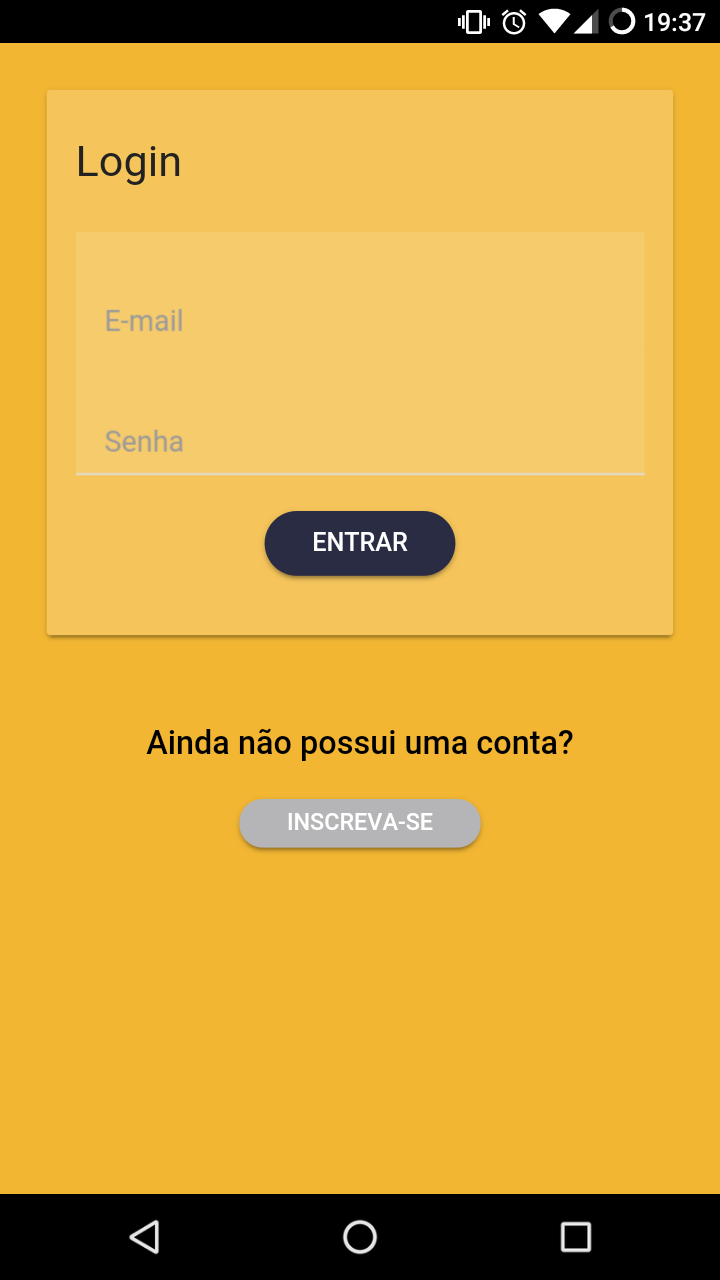
\includegraphics[scale=.55]{img/APP/login}}\qquad
    \subcaptionbox{\label{img:dados_atuais}Dados atuais}{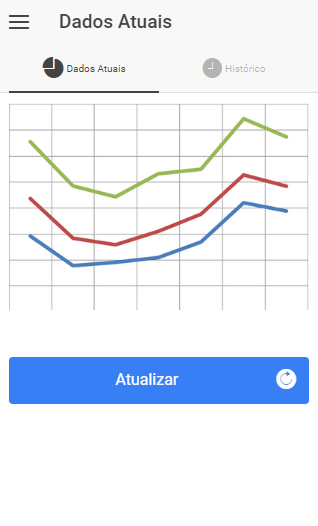
\includegraphics[scale=.55]{img/APP/dados_atuais}}\\
    \subcaptionbox{\label{img:hist-var}Escolher variáveis}{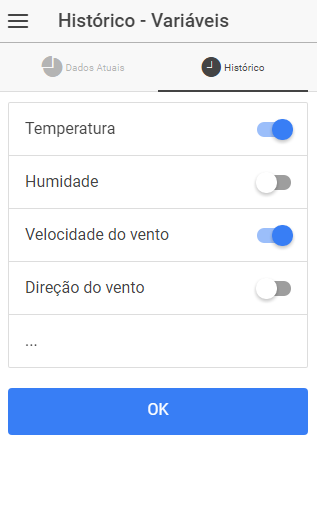
\includegraphics[scale=.55]{img/APP/hist-var}}\qquad
    \subcaptionbox{\label{img:hist-time}Seleção de período}{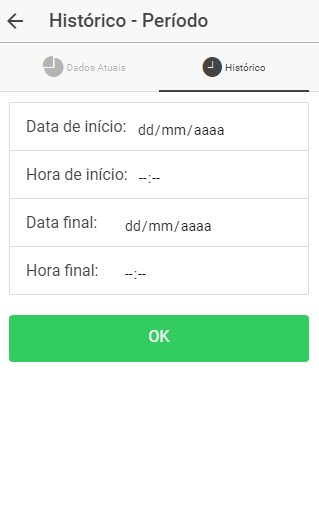
\includegraphics[scale=.55]{img/APP/hist-time}}\qquad
    \subcaptionbox{\label{img:hist-rel}Exibir histórico}{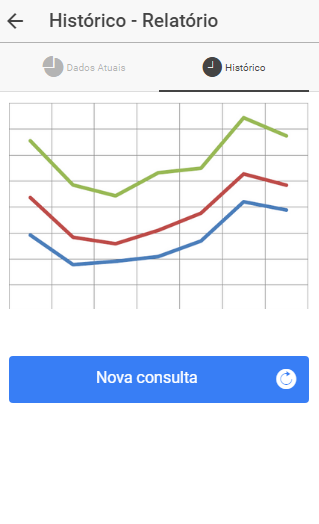
\includegraphics[scale=.55]{img/APP/hist-rel}}
    \legend{\textbf{Fonte:} O Autor}
\label{fig:dag}
\end{figure}

Além disso, será sempre permitido ao usuário retornar para a tela anterior através do botão voltar, com exceção da tela de \textit{login}, que só será acessível se o usuário realizar \textit{logoff} ou reiniciar a aplicação. O fluxo de funcionamento da aplicação cliente é representado pelo diagrama de atividades da figura \ref{img:atividades1} na subseção \ref{subsec:diagAtiv}.

A figura \ref{img:login} mostra a tela utilizada no caso de uso de autenticação do usuário. A figura \ref{img:dados_atuais} mostra a tela de visualização dos dados atuais. As figuras \ref{img:hist-var}, \ref{img:hist-time} e \ref{img:hist-rel} correspondem ao caso de uso de visualização de histórico.

É importante salientar que as telas aqui representadas são um protótipo, e durante a implementação do projeto podem sofrer alterações de \textit{design} e funcionalidades. Entretanto, já apresentam a ideia central de como será a aplicação.

\subsection{A API do sistema} \label{subsec:api}

Os URIs da API do sistema estão mostrados na tabela \ref{tab:api} abaixo. Assim como na subseção \ref{subsec:interfaceComOUsurario}, os identificadores aqui planejados são um protótipo e a medida que a implementação do sistema progride pode surgir a necessidade de alterá-los tanto sintaticamente quanto semânticamente. Assim como pode nascer a necessidade de adicionar novos identificadores ou de excluir algum dos planejados previamente.

A tabela divide-se em três partes, a primeira representa as ações que podem ser executadas por um usuário não autenticado, a segunda evidencia as ações possíveis para um usuário que efetuou \textit{login} e a terceira expõe as ações internas do sistema.

%\definecolor{Gray}{gray}{0.85}
\newpage

\begin{table}[!h]
\huge
\centering
\caption{\label{tab:api} API RESTful do sistema.}
\begin{adjustbox}{max width=\textwidth}
\begin{tabular}{@{} p{8.5cm} | l l p{10cm} @{}}
\toprule
%\rowcolor{Gray}
\multicolumn{1}{l}{Ator}                                 & Método & URI                                & Descrição                                                                                   \\ \hline
Usuário não autenticado              & POST   & /usuario/login                     & Autentica o usuário                                                                        ; \\ \hline
\multirow{5}{*}{Usuário autenticado} & GET    & /atual                             & Retorna o último documento da base de dados;                                                 \\ \cline{2-4}
                                     & GET    & /hist/\{id\_variavel\}/\{periodo\} & Retorna o histórico da variável no período especificado;                                     \\ \cline{2-4}
                                     & POST   & /usuario/novo                      & Cria um novo usuário com os parâmetros passados no corpo da requisição;                      \\ \cline{2-4}
                                     & PUT    & /usuario/\{username\}              & Atualiza os dados do usuário especificado com os parâmetros passados no corpo da requisição; \\ \cline{2-4}
                                     & DELETE & /usuario/\{username\}              & Deleta o usuário especificado;                                                               \\ \hline
\multirow{3}{*}{Sistema}             & POST   & /leitura                           & Cria um novo documento no banco os valores das variáveis passados no corpo da requisição;    \\ \cline{2-4}
                                     & DELETE & /leitura/\{id\}                    & Deleta a especificada leitura da base de dados;                                              \\ \cline{2-4}
                                     & PUT    & /leitura/\{id\}                    & Atualiza os dados da leitura especificada com os parâmetros passados no corpo da requisição; \\ %\cmidrule(l){2-4}
\bottomrule
                                      
\end{tabular}
\end{adjustbox}
\legend{\textbf{Fonte:} O Autor}
\end{table}





\subsection{Modelo de dados do sistema} \label{subsec:datamodel}

O banco de dados escolhido para a implementação do projeto é não-relacional baseado em documentos. Os documentos podem conter vários pares chave-valor, ou vários pares chave-vetor, ou até vários documentos encadeados. A estrutura do documento é flexível, o que permite alterações e inserções futuras de dados novos em uma base preexistente \cite{SITEMONGODB}. O modelo de dados inicial adotado para o projeto é mostrado na figura \ref{img:collection} abaixo, onde de um lado têm-se as chaves representando os dados fornecidos pela estação e do outro seus respectivos valores.

\imagem{0.55}{collection}{Modelo de documento do sistema}{O Autor}
\newpage

Os valores de cada chave adotada para o modelo de documentos são providos pelo \textit{datalogger} da estação. Algumas chaves possuem o valor obtido diretamente dos sensores, por exemplo a direção do vento. Em outros casos, os valores são calculados pela própria estação através de equações utilizando os dados derivados dos sensores, como por exemplo o ponto de orvalho, que faz uso da temperatura e da umidade externa em seu cálculo \cite{SITEVARIAVEIS}.
